\documentclass[sigconf,authorversion,nonacm]{acmart}

\AtBeginDocument{%
  \providecommand\BibTeX{{%
    \normalfont B\kern-0.5em{\scshape i\kern-0.25em b}\kern-0.8em\TeX}}}
\usepackage{hyperref}

\begin{document}

\settopmatter{printacmref=false}

\title{Internet weather maps and statistics: Which ones exist?}

\author{Bashar Khoulani}
\email{bashar@uni-kassel.de}
\affiliation{
  \institution{Universität Kassel - Distributed Systems}
  \city{Kassel}
  \state{Hessen}
  \country{Germany}
}

\begin{abstract}
Internet weather maps and statistics are tools that provide institutions with insightful information about their networks, applications, benefits, and limitations, e.g. the bandwidth between two devices, packet frame sizes, or temporal events. They can help with detecting congestions, anomalies and analyzing recurring events --- among other useful things. 

In this paper, I will discuss the background of Internet weather maps and statistics, their advantages (or disadvantages), and refer to Internet weather maps that currently exist.
\end{abstract}
\maketitle
\section{Introduction}
An Internet weather map consists of a network map and bandwidth measurements that lay out the structure and connections between the devices. A network undergoes several events and anomalies that weather maps can help detect. Network administrators can then discover the cause and mitigate the problems.

Statistics are (eventually aggregated) information that is collected over regular intervals to provide insights about the current usage of the network nodes and routers and to help detect peak events and possible anomalies. 

In the following section, some of the most common network issues will be mentioned and explained. 
\subsection{BACKGROUND}
\textbf{Congestion:} Network congestion reduces the quality of the network and is most often a temporary problem. The root cause is commonly a network node that processes data but more than it can handle. It is caused by insufficient bandwidth, poor network design, or node failures. Consequently, it delays processing packets, eventual packet loss, and overall network performance downgrade \cite{simulation}.

Several methods were developed to mitigate network congestion, such as RED (Random early detection), flow monitoring, and other protocols or algorithms embedded in switches and routers.

Random Early Detection (RED) is a network congestion avoidance mechanism. It constantly monitors data queue lengths at network routers, beginning to drop packets as queues grow, but in a probabilistic manner. This strategy cleverly signals data senders to decrease their transmission rate, effectively preempting potential congestion. RED's approach is similar to a traffic controller, incrementally increasing packet drop probabilities as queues approach critical levels, thus ensuring smoother network traffic flow. It balances network efficiency and congestion control, maintaining optimal data flow without abrupt interruptions \cite{251892}.

\textbf{Anomalies:} In large networks, some elements affect the day-to-day traffic which cannot be explained normally and are manifested as irregular traffic patterns, which differ significantly from the norms. They affect the network behavior and therefore it deviates from the standard behavior. These elements are called anomalies. 

With the help of weather maps and statistics, information about the anomalies' sources, dates, and time can be collected, which could eventually provide a conclusive explanation behind them. It is crucial to detect anomalies, due to some being malicious and caused by bot attacks \cite{6524462}. For example, sudden traffic spikes at odd hours may indicate a potential security breach, while gradual changes could indicate changing user behaviors or changes in network dynamics.

\section{Motivation and Ethics}
Many institutions deploy monitoring software on their networks to protect the infrastructure. The monitoring software and its output come close to Internet weather maps and statistics. On a global level, they introduce bigger benefits which could be several of the following:

\textbf{Intrusion and anomaly detection:} Internet weather maps and statistics can analyze the datasets collected through the network and identify patterns or trends that deviate from the norm. A sudden spike in traffic could mean a bot attack on the network, or an increase in latency could indicate a network congestion issue. With advanced techniques of graph theory and artificial intelligence, CDNs (Content Delivery Networks) can improve intrusion and anomaly detection to enhance network security.

\textbf{User experience:} Network providers can tailor content and make decisions on products or trends based on insights from Internet weather maps and statistics based on collected large datasets about interactions and time spent on selected websites. This helps identify trends, such as Internet usage in a weather season like winter or spring, optimizing resource allocation, or improving overall user satisfaction.

\textbf{Network management:} Internet weather maps and statistics can also be useful tools to analyze the needs of the network and attend to its maintenance. In this manner, potential bottlenecks and network requirements can be identified and handled in time, like predicting capacity bottlenecks and hardware failures. Furthermore, it can help optimize and organize network performance and use network resources efficiently. This is particularly important for CDNs, where efficient and on-time content delivery is vital. 

\textbf{Users' privacy:} As a sole disadvantage, one could argue that the privacy of the users, more precisely their payload or IP and MAC addresses, is at risk by deploying weather maps and statistics. They prove to be more at risk if the collected datasets are to be published for research purposes. Therefore, the datasets need to be cleaned and anonymized, their payload must be removed and the addresses should be scrambled so that the users cannot be identified, which requires manpower and resources \cite{271335}.

Overall, Internet weather maps and statistics mark a new era in network administration. They transform raw data into insightful information that leads to informative, smart, and knowledgeable actions.

\section{Related works}
This section will refer to several existing Internet weather maps and statistics and their research contributions.
\begin{figure}
    \centering
    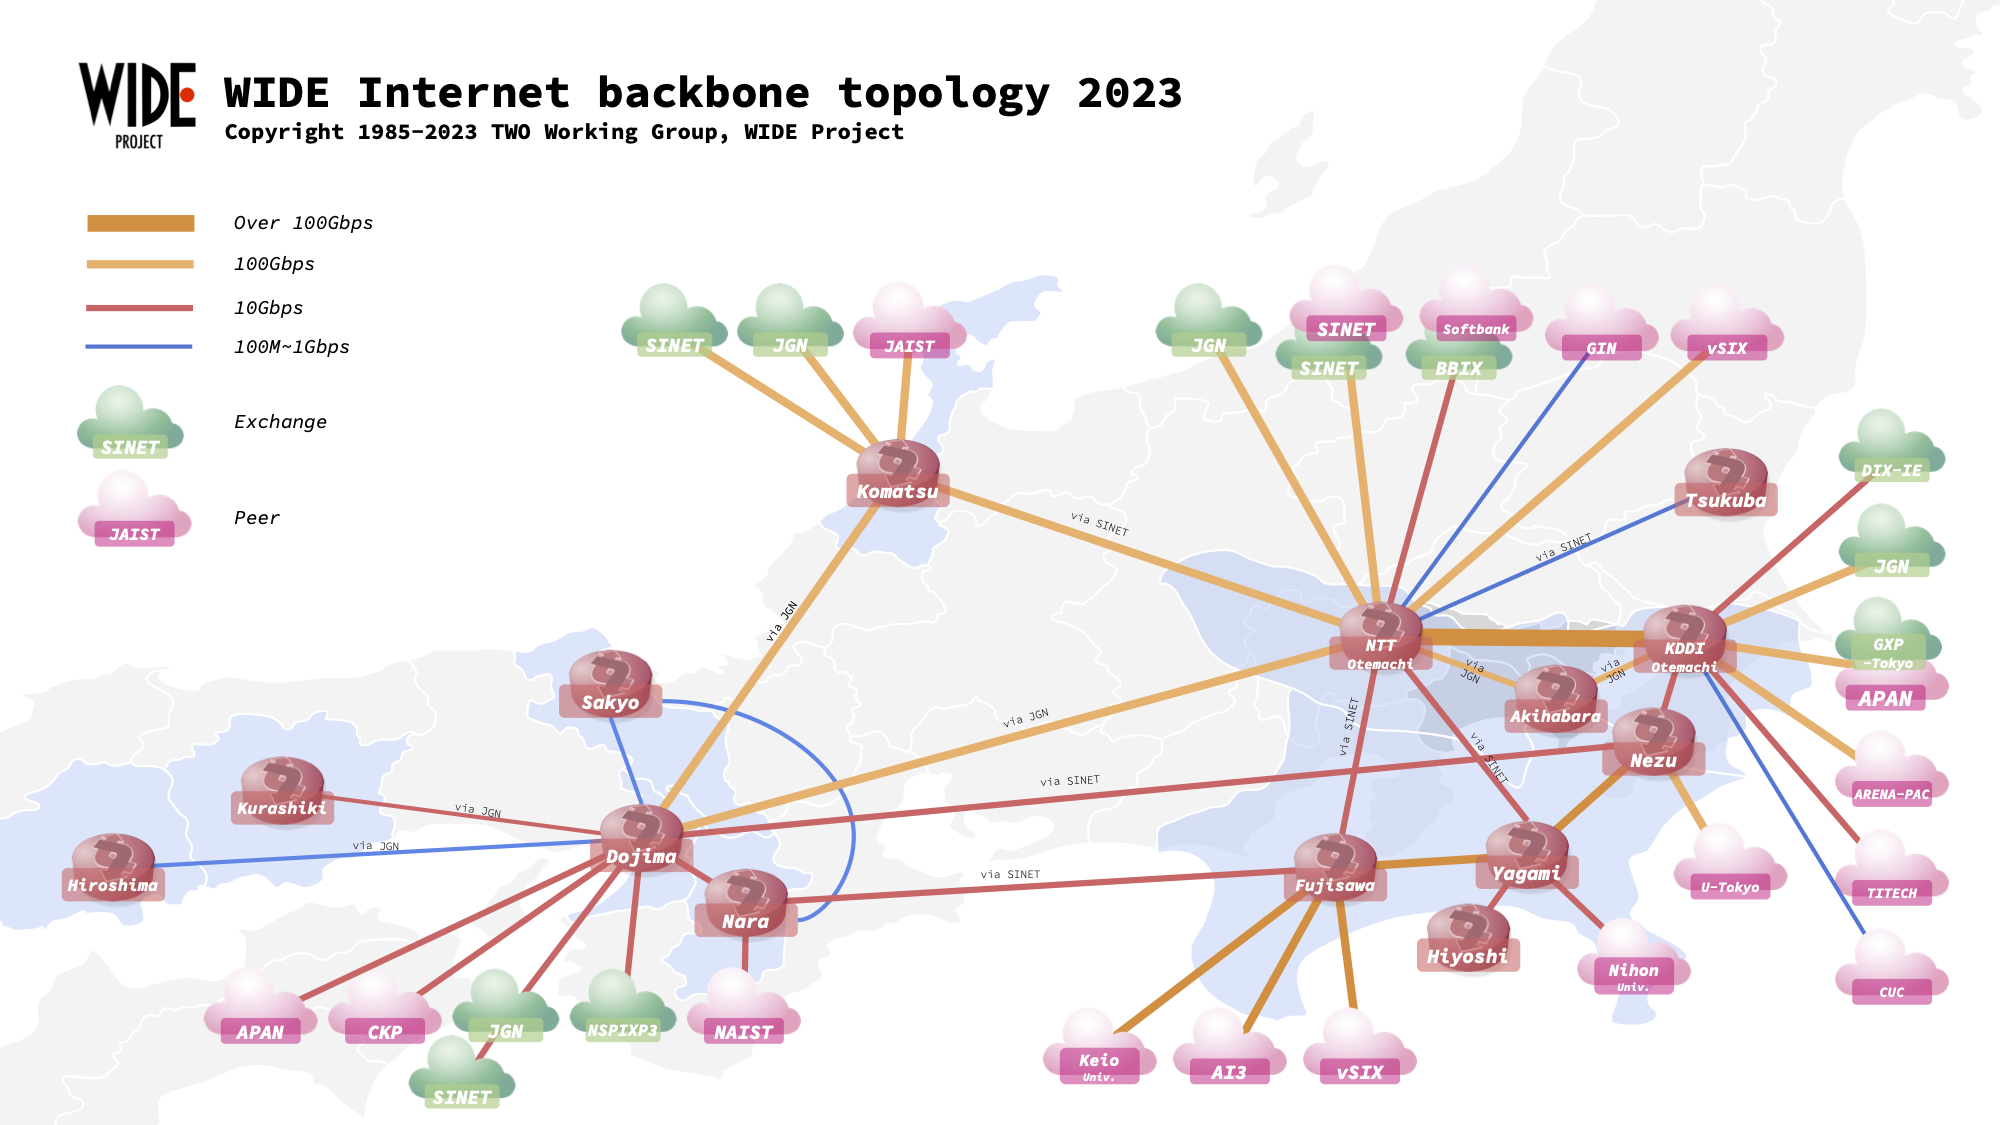
\includegraphics[width=\linewidth]{widebb-202309.png}
    \caption{WIDE Internet backbone topology 2023}
    \label{MAWI: WIDE Internet backbone topology 2023}
\end{figure}

\subsection{MAWI} The MAWI (Measurement and Analysis on the WIDE Internet \cite{271335}) Working Group is a collaborative effort by multiple Japanese network research and academic institutions. It stands at the forefront of network research, delivering invaluable insights into the backbone infrastructure of Japan. The WIDE network (AS2500) has the topology map as shown in figure \ref{MAWI: WIDE Internet backbone topology 2023}. It was operated to study networks and networking protocols in the Japanese network's backbone infrastructure and trans-Pacific backbone links. MAWI is one of the most known Internet weather maps and statistics sources, as its traffic archive was widely used as the basis of network research and has been in operation since 1999 until now (with some minor interruptions). This leads to exhaustive research methodologies to be applied, i.e. longitudinal studies.

The source code of the set of tools and the data repository are open source \footnote{\url{https://mawi.wide.ad.jp/mawi/}}. Packet traces are collected by the network traffic monitoring software tcpdump\footnote{\url{https://www.tcpdump.org/}} and anonymized with a modified version of tcpdriv\footnote{\url{https://ita.ee.lbl.gov/html/contrib/tcpdpriv.html}}. Network tracing starts every day from 14:00 until 14:15 (Japanese Standard Time, UTC+9). The packet traces are collected and made public at the data repository and are highly aggregated. A 15-minute long trace contains approximately 300k-500k unique IP addresses \cite{5061979}. The MAWI Working Group holds several sample points from the WIDE backbone infrastructure, of which sample point \textbf{B} and sample point \textbf{F} are the largest datasets. Sample point \textbf{B} was collected from January 2001 to June 2006, meanwhile, sample point \textbf{F} data was collected from October 2006 onwards. The sample point \textbf{F} monitors a 1Gb/s transport link from Tokyo to the NTT Global IP Network (AS2914). Traffic on the link was port mirrored to a 10Gb/s link on the router and captured using a commodity PC server and a 10GbE NIC running FreeBSD. Different sample points originate due to different settings and newer or older links. An example trace from sample point \textbf{F} was taken on December 10, 2023, and is to be analyzed in the following \cite{traceMAWI}:

\begin{figure}
        \centering
        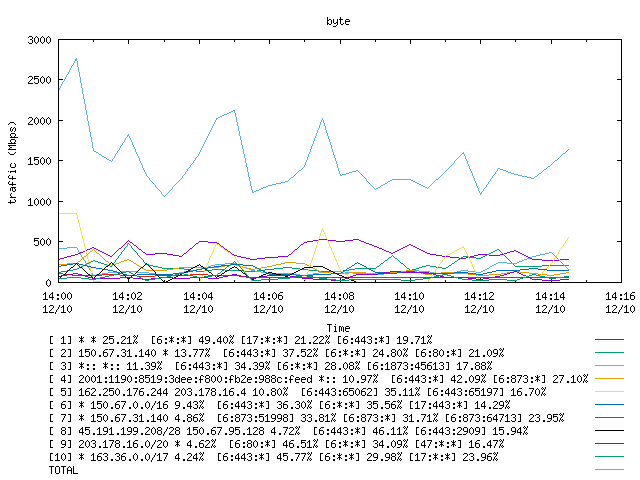
\includegraphics[width=1\linewidth]{MAWI 2023-12-10 aggregated analysis byte.png}
        \caption{MAWI: Aggregated flow of traffic}
        \label{MAWI: Aggregated Flow Byte}
\end{figure}

The figures \ref{MAWI: Aggregated Flow Byte} and \ref{MAWI: Aggregated Flow Packet} show the aggregated flow summary of the traffic flow at the WIDE Internet:

Figure \ref{MAWI: Aggregated Flow Byte} shows the stream of several connections that are ranked below the graph based on their percentages of the total traffic. The graph illustrates the changes in the traffic stream in Mbps over time. As an example, the connection ranked second is in IPv4 protocol and is from the source address 150.67.31.140 and the destination address is the wildcard * (in this case 0.0.0.0/0 for IPv4). It had a total usage of 13.77\%. The same connection has statistical information on the used protocols and ports and their percentages of the traffic at that connection. For example, the connection had 37.52\% of traffic using the Internet protocol TCP (Transmission Control Protocol) (based on Assigned Internet Protocol Numbers) on HTTPS (Hypertext Transfer Protocol Secure). The destination port is the wildcard *, which stands for any port in the destination \cite{179442}.

\begin{figure}
        \centering
        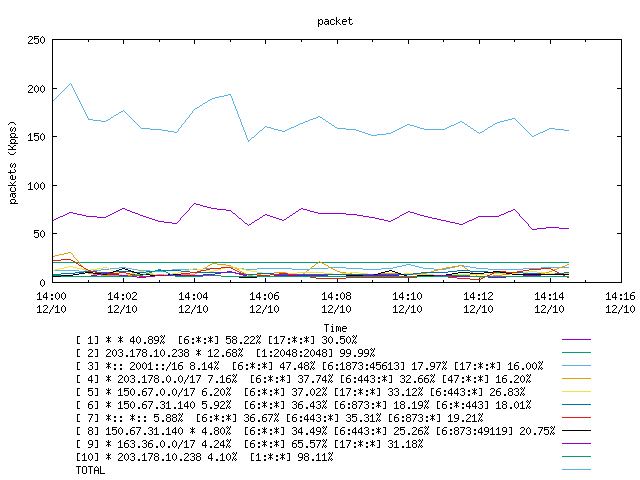
\includegraphics[width=1\linewidth]{MAWI 2023-12-10 aggregated analysis packet.png}
        \caption{MAWI: Aggregated flow of packets}
        \label{MAWI: Aggregated Flow Packet}
\end{figure}

Figure \ref{MAWI: Aggregated Flow Packet} illustrates the change in Kilo packets per second over time from the connections ranked in the top ten based on their traffic percentage. The syntax of the connections text below the graph is identical to those from figure \ref{MAWI: Aggregated Flow Byte}. Furthermore, the graph displays a connection stream in the color green that is constant over time. This originates from the USC ANT project\footnote{\url{https://ant.isi.edu/address/}} for probing the IPv4 space.

Both figures provide substantial information on how the traffic changes over time, especially when combined with other traffic traces. Case studies can be made possible on individual times through specific days and attacks and anomalies can be identified faster and more efficiently using the collected traces.

The MAWI data repository is open to the public, records real public data which allows them to publish them freely, and supports IPv4 and IPv6. Therefore, the traffic traces must undergo anonymization to protect the users' privacy. A guideline for users' privacy protection has been set in force by the MAWI Working Group, such that data sets can be used in research without privacy concerns\footnote{\url{https://mawi.wide.ad.jp/mawi/guideline.txt}}:

The first rule in the MAWI guideline is to remove any payload the traffic traces have received. TCP and UDP protocols are rid of their payload, and if there exist packets with another protocol on top, and the inner packet header does not have any private user information, then the inner packet header is not removed. The second rule is to scramble source and destination addresses based on two methods. The first method is to map an IP address to a different IP address using a hash function. The second method is used if two IP addresses have a common address prefix, then both are mapped to addresses with a common address prefix of the same length. Addresses lacking user identifiers must not be scrambled, e.g. broadcast, multicast, and private addresses. In IPv6 mode, link-local addresses and site-local addresses should be scrambled, because they could contain user MAC addresses. Aside from that, Ethernet headers also do not have to be scrambled due to them being the internal nodes', in other words, backbone networks' addresses.

The MAWI Working Group suggests in the guideline three different scrambling policies for consistency, where the guideline recommends the second option:
\begin{itemize}
    \item A TCP session in a single data set is mapped to the same address. 
    \item All occurrences of addresses in a data set are scrambled to a single address.
    \item All occurrences of addresses in several data sets are scrambled to a single address.
\end{itemize}

As a result of following the guidelines, the privacy of the end-users at the WIDE project is guaranteed and the risk of revealing sensitive information is kept at a minimum. Therefore, the MAWI dataset can be used for research without compromising user confidentiality.

Several real-world applications emerged from the MAWI archive to help network researchers in their studies on anomaly detection. For instance, MAWILab\footnote{\url{http://www.fukuda-lab.org/mawilab/}} is a project database that assists researchers in evaluating traffic anomaly detection methods. MAWILab uses both sample points \textbf{B} and \textbf{F} that are mentioned above. Furthermore, the database is updated daily to include new traffic traces and possible anomalies \cite{mawilab}. 

\begin{figure}
        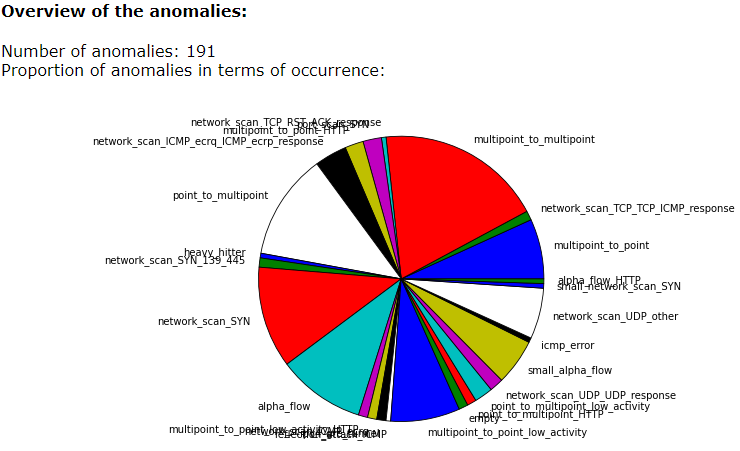
\includegraphics[width=\linewidth]{mawilab.PNG}
        \caption{MAWILab Anomaly Detection Overview}
        \label{MAWI: MAWILab Anomaly Detection Overview}
\end{figure}

In the figure \ref{MAWI: MAWILab Anomaly Detection Overview}, MAWILab provides anomaly detection analysis for a specific trace on August 2, 2023, from the MAWI archive\footnote{\url{http://www.fukuda-lab.org/mawilab/v1.1/2023/08/02/20230802.html}}. It detected 191 anomalies, of which several were network scans or multipoint-to-multipoint connections. MAWILab also provides a detailed table of all anomalies, with attributes like source or destination IP address, source or destination port, and what type of taxonomy was used, as shown in \ref{anomaly} (some columns were removed for better visibility, e.g. source port, destination IP address, and so on).

\begin{table}[!ht]
    \centering
    \caption{MAWI: Anomalies in trace of August 2, 2023}
    \label{anomaly}
    \begin{tabular}{|l|l|l|l|l|l|l|}
    \hline
        anomalyID &  srcIP & dstPort & nbDetectors \\ \hline
        109 & 185.233.188.247 & 22 & anomalous \\ \hline
        110 & 183.112.233.74 & 22 & anomalous \\ \hline
        113 & 119.160.59.14 & 6379 & anomalous \\ \hline
        114 & 81.73.84.186 & 6379 & anomalous \\ \hline
        116 & 188.93.176.191 & 2048 & anomalous \\ \hline
        116 & 188.93.176.191 & 49152 & anomalous \\ \hline
    \end{tabular}
\end{table}

Additionally, two longitudinal analyses were made possible by the MAWI Working Group due to its preserving, archived, and up-to-date datasets as of the current date. Longitudinal analyses refer to studies where observations are made over an extended period. They assess changes and developments of underlying structures, paving the way for understanding long-term trends and patterns. 

The first longitudinal analysis is a comprehensive seven-year study that reveals significant day-to-day variability which is influenced by congestion and random anomalies. Therefore, no conclusive remarks can be made about the long-term evolutions of network traffic. Nonetheless, authors were able to develop methodological approaches to prevent day-to-day incidental variabilities by utilizing sketches and median averages, hence enhancing the reliability of traffic estimation and focusing on long-term evolution. Moreover, the study shows that Internet traffic remained stable over the entire period \cite{5061979}. 

The second longitudinal analysis was made after fourteen years of the foundation of the MAWI Working Group. The 14-year longitudinal study on Internet (MAWI) traffic highlights two main scaling ranges in Internet traffic - coarse and fine scales, i.e. smaller and bigger versions of traffic. This indicates a consistent biscaling system across time, despite technological evolution. At coarse scales, long-range dependence (LRD) accurately depicts the traffic dynamics. Conversely, at fine scales, multifractal properties are more descriptive, contributing to the observed temporal burstiness in Internet traffic \cite{7878657}.

Overall, it is safe to say that the MAWI Working Group has been a tremendous help to the networking community providing helpful tools such as agurim and tcpdpriv, and the data repository itself for research purposes. The datasets have laid a good structure by delivering continuous traces and anonymizing them in the process. 

\subsection{OVH}
OVH is a French cloud computing company that offers virtual private or dedicated servers and other web services. It counts as one of the largest hosting providers in the world, spanning over 40 data centers in 9 countries across the world. They possess the autonomous system number 16276\footnote{\url{https://www.peeringdb.com/net/1264}}.

\begin{figure}[H]
    \centering
    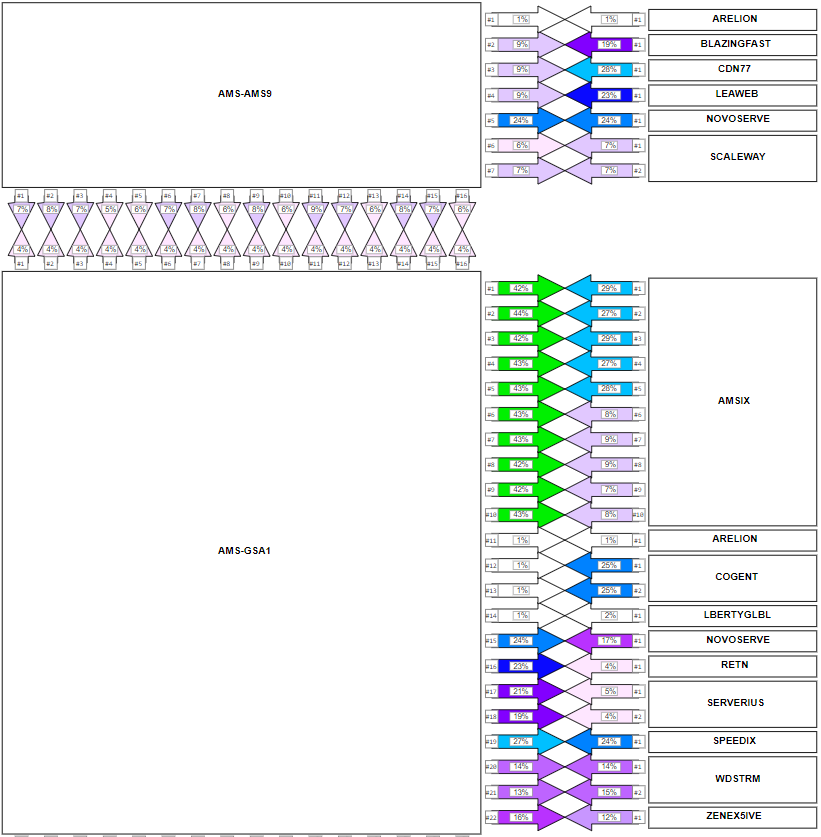
\includegraphics[width=\linewidth]{ovh.png}
    \caption{OVH: Excerpt from the European backbone network}
    \label{OVH: Excerpt from the European backbone network}
\end{figure}
OVH hosts their Internet weather map, providing information about their OVH data centers, peers, and load of each link between peers and data centers\footnote{\url{http://weathermap.ovh.net/}}. In figure \ref{OVH: Excerpt from the European backbone network}, Global Switch and Digital Realty data centers in Amsterdam are illustrated as a big rectangle, meanwhile, peers are pictured on the side as smaller rectangles. Links (Out- and ongoing bandwidth) are depicted as arrows going out from the respective rectangle. For example, the Amsterdam Internet Exchange has 10 parallel links connected with the Global Switch data center. The arrows are colored based on their bandwidth loads that follow the criteria in figure \ref{OVH: Links bandwidth load scale}.
\begin{figure}[H]
    \centering
    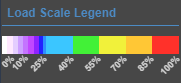
\includegraphics{scale.png}
    \caption{OVH: Links bandwidth load scale}
    \label{OVH: Links bandwidth load scale}
\end{figure}
\section{Conclusion}

\bibliographystyle{ACM-Reference-Format}
\bibliography{sample-base}

\appendix

\section{Manda}
What are Internet Weathermaps?
How can they be useful?
Which ones exist?
The first two questions are the motivation behind the work and the main focus should be on finding out which Internet weathermaps exist.
Manda

https://www.seattleix.net/statistics/

https://gist.github.com/stefanbschneider/96602bb3c8b256b90058d59f337a0e59


\end{document}